\documentclass[1p]{elsarticle_modified}
%\bibliographystyle{elsarticle-num}

%\usepackage[colorlinks]{hyperref}
%\usepackage{abbrmath_seonhwa} %\Abb, \Ascr, \Acal ,\Abf, \Afrak
\usepackage{amsfonts}
\usepackage{amssymb}
\usepackage{amsmath}
\usepackage{amsthm}
\usepackage{scalefnt}
\usepackage{amsbsy}
\usepackage{kotex}
\usepackage{caption}
\usepackage{subfig}
\usepackage{color}
\usepackage{graphicx}
\usepackage{xcolor} %% white, black, red, green, blue, cyan, magenta, yellow
\usepackage{float}
\usepackage{setspace}
\usepackage{hyperref}

\usepackage{tikz}
\usetikzlibrary{arrows}

\usepackage{multirow}
\usepackage{array} % fixed length table
\usepackage{hhline}

%%%%%%%%%%%%%%%%%%%%%
\makeatletter
\renewcommand*\env@matrix[1][\arraystretch]{%
	\edef\arraystretch{#1}%
	\hskip -\arraycolsep
	\let\@ifnextchar\new@ifnextchar
	\array{*\c@MaxMatrixCols c}}
\makeatother %https://tex.stackexchange.com/questions/14071/how-can-i-increase-the-line-spacing-in-a-matrix
%%%%%%%%%%%%%%%

\usepackage[normalem]{ulem}

\newcommand{\msout}[1]{\ifmmode\text{\sout{\ensuremath{#1}}}\else\sout{#1}\fi}
%SOURCE: \msout is \stkout macro in https://tex.stackexchange.com/questions/20609/strikeout-in-math-mode

\newcommand{\cancel}[1]{
	\ifmmode
	{\color{red}\msout{#1}}
	\else
	{\color{red}\sout{#1}}
	\fi
}

\newcommand{\add}[1]{
	{\color{blue}\uwave{#1}}
}

\newcommand{\replace}[2]{
	\ifmmode
	{\color{red}\msout{#1}}{\color{blue}\uwave{#2}}
	\else
	{\color{red}\sout{#1}}{\color{blue}\uwave{#2}}
	\fi
}

\newcommand{\Sol}{\mathcal{S}} %segment
\newcommand{\D}{D} %diagram
\newcommand{\A}{\mathcal{A}} %arc


%%%%%%%%%%%%%%%%%%%%%%%%%%%%%5 test

\def\sl{\operatorname{\textup{SL}}(2,\Cbb)}
\def\psl{\operatorname{\textup{PSL}}(2,\Cbb)}
\def\quan{\mkern 1mu \triangleright \mkern 1mu}

\theoremstyle{definition}
\newtheorem{thm}{Theorem}[section]
\newtheorem{prop}[thm]{Proposition}
\newtheorem{lem}[thm]{Lemma}
\newtheorem{ques}[thm]{Question}
\newtheorem{cor}[thm]{Corollary}
\newtheorem{defn}[thm]{Definition}
\newtheorem{exam}[thm]{Example}
\newtheorem{rmk}[thm]{Remark}
\newtheorem{alg}[thm]{Algorithm}

\newcommand{\I}{\sqrt{-1}}
\begin{document}

%\begin{frontmatter}
%
%\title{Boundary parabolic representations of knots up to 8 crossings}
%
%%% Group authors per affiliation:
%\author{Yunhi Cho} 
%\address{Department of Mathematics, University of Seoul, Seoul, Korea}
%\ead{yhcho@uos.ac.kr}
%
%
%\author{Seonhwa Kim} %\fnref{s_kim}}
%\address{Center for Geometry and Physics, Institute for Basic Science, Pohang, 37673, Korea}
%\ead{ryeona17@ibs.re.kr}
%
%\author{Hyuk Kim}
%\address{Department of Mathematical Sciences, Seoul National University, Seoul 08826, Korea}
%\ead{hyukkim@snu.ac.kr}
%
%\author{Seokbeom Yoon}
%\address{Department of Mathematical Sciences, Seoul National University, Seoul, 08826,  Korea}
%\ead{sbyoon15@snu.ac.kr}
%
%\begin{abstract}
%We find all boundary parabolic representation of knots up to 8 crossings.
%
%\end{abstract}
%\begin{keyword}
%    \MSC[2010] 57M25 
%\end{keyword}
%
%\end{frontmatter}

%\linenumbers
%\tableofcontents
%
\newcommand\colored[1]{\textcolor{white}{\rule[-0.35ex]{0.8em}{1.4ex}}\kern-0.8em\color{red} #1}%
%\newcommand\colored[1]{\textcolor{white}{ #1}\kern-2.17ex	\textcolor{white}{ #1}\kern-1.81ex	\textcolor{white}{ #1}\kern-2.15ex\color{red}#1	}

{\Large $\underline{12n_{0401}~(K12n_{0401})}$}

\setlength{\tabcolsep}{10pt}
\renewcommand{\arraystretch}{1.6}
\vspace{1cm}\begin{tabular}{m{100pt}>{\centering\arraybackslash}m{274pt}}
\multirow{5}{120pt}{
	\centering
	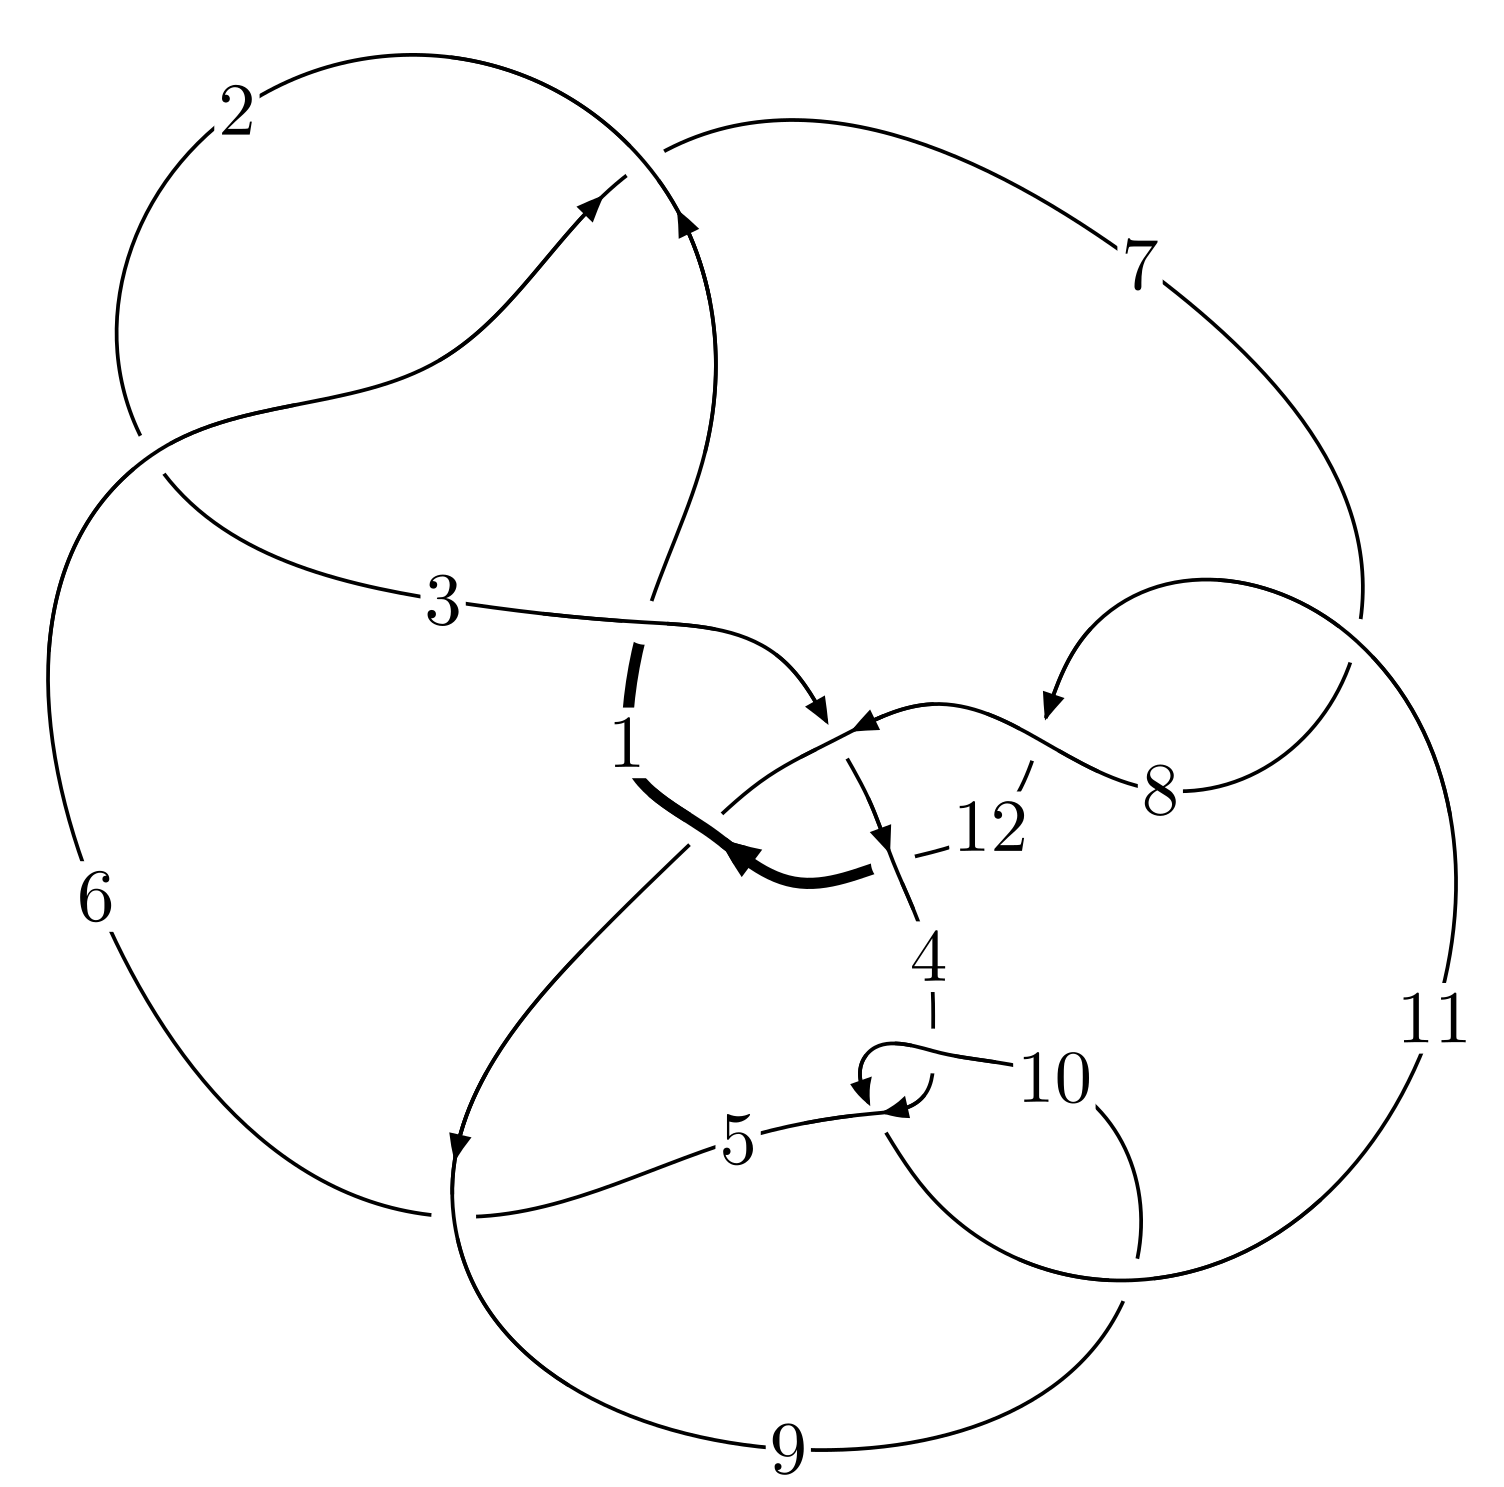
\includegraphics[width=112pt]{../../../GIT/diagram.site/Diagrams/png/2490_12n_0401.png}\\
\ \ \ A knot diagram\footnotemark}&
\allowdisplaybreaks
\textbf{Linearized knot diagam} \\
\cline{2-2}
 &
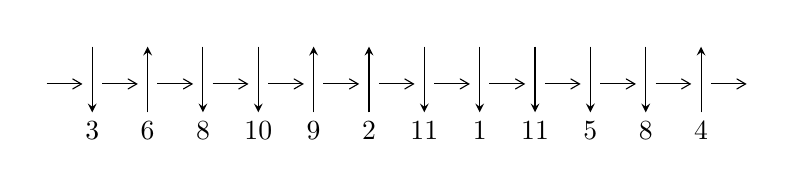
\begin{tikzpicture}[x=20pt, y=17pt]
	% nodes
	\node (C0) at (0, 0) {};
	\node (C1) at (1, 0) {};
	\node (C1U) at (1, +1) {};
	\node (C1D) at (1, -1) {3};

	\node (C2) at (2, 0) {};
	\node (C2U) at (2, +1) {};
	\node (C2D) at (2, -1) {6};

	\node (C3) at (3, 0) {};
	\node (C3U) at (3, +1) {};
	\node (C3D) at (3, -1) {8};

	\node (C4) at (4, 0) {};
	\node (C4U) at (4, +1) {};
	\node (C4D) at (4, -1) {10};

	\node (C5) at (5, 0) {};
	\node (C5U) at (5, +1) {};
	\node (C5D) at (5, -1) {9};

	\node (C6) at (6, 0) {};
	\node (C6U) at (6, +1) {};
	\node (C6D) at (6, -1) {2};

	\node (C7) at (7, 0) {};
	\node (C7U) at (7, +1) {};
	\node (C7D) at (7, -1) {11};

	\node (C8) at (8, 0) {};
	\node (C8U) at (8, +1) {};
	\node (C8D) at (8, -1) {1};

	\node (C9) at (9, 0) {};
	\node (C9U) at (9, +1) {};
	\node (C9D) at (9, -1) {11};

	\node (C10) at (10, 0) {};
	\node (C10U) at (10, +1) {};
	\node (C10D) at (10, -1) {5};

	\node (C11) at (11, 0) {};
	\node (C11U) at (11, +1) {};
	\node (C11D) at (11, -1) {8};

	\node (C12) at (12, 0) {};
	\node (C12U) at (12, +1) {};
	\node (C12D) at (12, -1) {4};
	\node (C13) at (13, 0) {};

	% arrows
	\draw[->,>={angle 60}]
	(C0) edge (C1) (C1) edge (C2) (C2) edge (C3) (C3) edge (C4) (C4) edge (C5) (C5) edge (C6) (C6) edge (C7) (C7) edge (C8) (C8) edge (C9) (C9) edge (C10) (C10) edge (C11) (C11) edge (C12) (C12) edge (C13) ;	\draw[->,>=stealth]
	(C1U) edge (C1D) (C2D) edge (C2U) (C3U) edge (C3D) (C4U) edge (C4D) (C5D) edge (C5U) (C6D) edge (C6U) (C7U) edge (C7D) (C8U) edge (C8D) (C9U) edge (C9D) (C10U) edge (C10D) (C11U) edge (C11D) (C12D) edge (C12U) ;
	\end{tikzpicture} \\
\hhline{~~} \\& 
\textbf{Solving Sequence} \\ \cline{2-2} 
 &
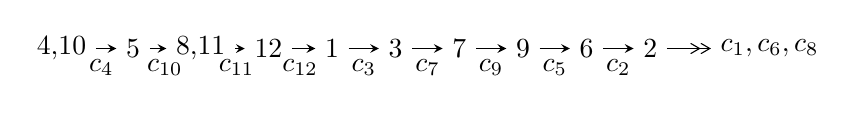
\begin{tikzpicture}[x=23pt, y=7pt]
	% node
	\node (A0) at (-1/8, 0) {4,10};
	\node (A1) at (1, 0) {5};
	\node (A2) at (33/16, 0) {8,11};
	\node (A3) at (25/8, 0) {12};
	\node (A4) at (33/8, 0) {1};
	\node (A5) at (41/8, 0) {3};
	\node (A6) at (49/8, 0) {7};
	\node (A7) at (57/8, 0) {9};
	\node (A8) at (65/8, 0) {6};
	\node (A9) at (73/8, 0) {2};
	\node (C1) at (1/2, -1) {$c_{4}$};
	\node (C2) at (3/2, -1) {$c_{10}$};
	\node (C3) at (21/8, -1) {$c_{11}$};
	\node (C4) at (29/8, -1) {$c_{12}$};
	\node (C5) at (37/8, -1) {$c_{3}$};
	\node (C6) at (45/8, -1) {$c_{7}$};
	\node (C7) at (53/8, -1) {$c_{9}$};
	\node (C8) at (61/8, -1) {$c_{5}$};
	\node (C9) at (69/8, -1) {$c_{2}$};
	\node (A10) at (11, 0) {$c_{1},c_{6},c_{8}$};

	% edge
	\draw[->,>=stealth]	
	(A0) edge (A1) (A1) edge (A2) (A2) edge (A3) (A3) edge (A4) (A4) edge (A5) (A5) edge (A6) (A6) edge (A7) (A7) edge (A8) (A8) edge (A9) ;
	\draw[->>,>={angle 60}]	
	(A9) edge (A10);
\end{tikzpicture} \\ 

\end{tabular} \\

\footnotetext{
The image of knot diagram is generated by the software ``\textbf{Draw programme}" developed by Andrew Bartholomew(\url{http://www.layer8.co.uk/maths/draw/index.htm\#Running-draw}), where we modified some parts for our purpose(\url{https://github.com/CATsTAILs/LinksPainter}).
}\phantom \\ \newline 
\centering \textbf{Ideals for irreducible components\footnotemark of $X_{\text{par}}$} 
 
\begin{align*}
I^u_{1}&=\langle 
9.38926\times10^{46} u^{60}-4.46475\times10^{46} u^{59}+\cdots+4.27875\times10^{46} b-7.71448\times10^{47},\\
\phantom{I^u_{1}}&\phantom{= \langle  }-5.92525\times10^{47} u^{60}+3.42901\times10^{47} u^{59}+\cdots+2.99512\times10^{47} a+4.84559\times10^{48},\;u^{61}- u^{60}+\cdots-4 u+7\rangle \\
I^u_{2}&=\langle 
u^{17}-4 u^{15}+9 u^{13}-11 u^{11}+u^{10}+9 u^9-3 u^8-2 u^7+4 u^6-2 u^5-2 u^4+4 u^3+b- u,\\
\phantom{I^u_{2}}&\phantom{= \langle  }-2 u^{17}+u^{16}+8 u^{15}-4 u^{14}-17 u^{13}+8 u^{12}+19 u^{11}-10 u^{10}-11 u^9+10 u^8-4 u^7-6 u^6+9 u^5-5 u^3+3 u^2+a,\\
\phantom{I^u_{2}}&\phantom{= \langle  }u^{18}-5 u^{16}+13 u^{14}-20 u^{12}+u^{11}+20 u^{10}-4 u^9-11 u^8+7 u^7+u^6-6 u^5+4 u^4+2 u^3-3 u^2+1\rangle \\
\\
\end{align*}
\raggedright * 2 irreducible components of $\dim_{\mathbb{C}}=0$, with total 79 representations.\\
\footnotetext{All coefficients of polynomials are rational numbers. But the coefficients are sometimes approximated in decimal forms when there is not enough margin.}
\newpage
\renewcommand{\arraystretch}{1}
\centering \section*{I. $I^u_{1}= \langle 9.39\times10^{46} u^{60}-4.46\times10^{46} u^{59}+\cdots+4.28\times10^{46} b-7.71\times10^{47},\;-5.93\times10^{47} u^{60}+3.43\times10^{47} u^{59}+\cdots+3.00\times10^{47} a+4.85\times10^{48},\;u^{61}- u^{60}+\cdots-4 u+7 \rangle$}
\flushleft \textbf{(i) Arc colorings}\\
\begin{tabular}{m{7pt} m{180pt} m{7pt} m{180pt} }
\flushright $a_{4}=$&$\begin{pmatrix}1\\0\end{pmatrix}$ \\
\flushright $a_{10}=$&$\begin{pmatrix}0\\u\end{pmatrix}$ \\
\flushright $a_{5}=$&$\begin{pmatrix}1\\u^2\end{pmatrix}$ \\
\flushright $a_{8}=$&$\begin{pmatrix}1.97830 u^{60}-1.14487 u^{59}+\cdots-9.80742 u-16.1783\\-2.19440 u^{60}+1.04347 u^{59}+\cdots+9.97369 u+18.0298\end{pmatrix}$ \\
\flushright $a_{11}=$&$\begin{pmatrix}- u\\- u^3+u\end{pmatrix}$ \\
\flushright $a_{12}=$&$\begin{pmatrix}2.02259 u^{60}-1.64099 u^{59}+\cdots-13.4590 u-21.6582\\-0.378227 u^{60}+0.935730 u^{59}+\cdots+11.4450 u+10.1138\end{pmatrix}$ \\
\flushright $a_{1}=$&$\begin{pmatrix}1.64436 u^{60}-0.705262 u^{59}+\cdots-2.01406 u-11.5444\\-0.378227 u^{60}+0.935730 u^{59}+\cdots+11.4450 u+10.1138\end{pmatrix}$ \\
\flushright $a_{3}=$&$\begin{pmatrix}-0.129915 u^{60}+0.492637 u^{59}+\cdots+13.1288 u+10.6244\\-0.000539469 u^{60}+0.281363 u^{59}+\cdots+2.40949 u+4.06086\end{pmatrix}$ \\
\flushright $a_{7}=$&$\begin{pmatrix}2.95189 u^{60}-1.23072 u^{59}+\cdots-6.85929 u-18.3643\\-2.29268 u^{60}+0.793366 u^{59}+\cdots+3.76139 u+14.0016\end{pmatrix}$ \\
\flushright $a_{9}=$&$\begin{pmatrix}u^3\\u^5- u^3+u\end{pmatrix}$ \\
\flushright $a_{6}=$&$\begin{pmatrix}u^6- u^4+1\\u^8-2 u^6+2 u^4\end{pmatrix}$ \\
\flushright $a_{2}=$&$\begin{pmatrix}0.888507 u^{60}+0.465150 u^{59}+\cdots+15.6860 u+5.85422\\0.416055 u^{60}-0.229418 u^{59}+\cdots-3.73540 u-1.33752\end{pmatrix}$\\&\end{tabular}
\flushleft \textbf{(ii) Obstruction class $= -1$}\\~\\
\flushleft \textbf{(iii) Cusp Shapes $= 8.30801 u^{60}+0.834443 u^{59}+\cdots+12.8461 u-49.4860$}\\~\\
\newpage\renewcommand{\arraystretch}{1}
\flushleft \textbf{(iv) u-Polynomials at the component}\newline \\
\begin{tabular}{m{50pt}|m{274pt}}
Crossings & \hspace{64pt}u-Polynomials at each crossing \\
\hline $$\begin{aligned}c_{1}\end{aligned}$$&$\begin{aligned}
&u^{61}+22 u^{60}+\cdots-10584 u-841
\end{aligned}$\\
\hline $$\begin{aligned}c_{2},c_{6}\end{aligned}$$&$\begin{aligned}
&u^{61}-2 u^{60}+\cdots-28 u+29
\end{aligned}$\\
\hline $$\begin{aligned}c_{3}\end{aligned}$$&$\begin{aligned}
&u^{61}- u^{60}+\cdots+4065 u+1393
\end{aligned}$\\
\hline $$\begin{aligned}c_{4},c_{10}\end{aligned}$$&$\begin{aligned}
&u^{61}- u^{60}+\cdots-4 u+7
\end{aligned}$\\
\hline $$\begin{aligned}c_{5}\end{aligned}$$&$\begin{aligned}
&u^{61}-3 u^{60}+\cdots-11403 u+4312
\end{aligned}$\\
\hline $$\begin{aligned}c_{7},c_{11}\end{aligned}$$&$\begin{aligned}
&u^{61}+36 u^{59}+\cdots+207224 u+19571
\end{aligned}$\\
\hline $$\begin{aligned}c_{8}\end{aligned}$$&$\begin{aligned}
&u^{61}+3 u^{60}+\cdots+7 u+2
\end{aligned}$\\
\hline $$\begin{aligned}c_{9}\end{aligned}$$&$\begin{aligned}
&u^{61}+27 u^{60}+\cdots+324 u+49
\end{aligned}$\\
\hline $$\begin{aligned}c_{12}\end{aligned}$$&$\begin{aligned}
&u^{61}+7 u^{60}+\cdots+119062 u+4921
\end{aligned}$\\
\hline
\end{tabular}\\~\\
\newpage\renewcommand{\arraystretch}{1}
\flushleft \textbf{(v) Riley Polynomials at the component}\newline \\
\begin{tabular}{m{50pt}|m{274pt}}
Crossings & \hspace{64pt}Riley Polynomials at each crossing \\
\hline $$\begin{aligned}c_{1}\end{aligned}$$&$\begin{aligned}
&y^{61}+58 y^{60}+\cdots+53870952 y-707281
\end{aligned}$\\
\hline $$\begin{aligned}c_{2},c_{6}\end{aligned}$$&$\begin{aligned}
&y^{61}+22 y^{60}+\cdots-10584 y-841
\end{aligned}$\\
\hline $$\begin{aligned}c_{3}\end{aligned}$$&$\begin{aligned}
&y^{61}+73 y^{60}+\cdots-72881301 y-1940449
\end{aligned}$\\
\hline $$\begin{aligned}c_{4},c_{10}\end{aligned}$$&$\begin{aligned}
&y^{61}-27 y^{60}+\cdots+324 y-49
\end{aligned}$\\
\hline $$\begin{aligned}c_{5}\end{aligned}$$&$\begin{aligned}
&y^{61}-15 y^{60}+\cdots+131313385 y-18593344
\end{aligned}$\\
\hline $$\begin{aligned}c_{7},c_{11}\end{aligned}$$&$\begin{aligned}
&y^{61}+72 y^{60}+\cdots+1955728272 y-383024041
\end{aligned}$\\
\hline $$\begin{aligned}c_{8}\end{aligned}$$&$\begin{aligned}
&y^{61}-7 y^{60}+\cdots-103 y-4
\end{aligned}$\\
\hline $$\begin{aligned}c_{9}\end{aligned}$$&$\begin{aligned}
&y^{61}+21 y^{60}+\cdots+6192 y-2401
\end{aligned}$\\
\hline $$\begin{aligned}c_{12}\end{aligned}$$&$\begin{aligned}
&y^{61}-73 y^{60}+\cdots+2203035738 y-24216241
\end{aligned}$\\
\hline
\end{tabular}\\~\\
\newpage\flushleft \textbf{(vi) Complex Volumes and Cusp Shapes}
$$\begin{array}{c|c|c}  
\text{Solutions to }I^u_{1}& \I (\text{vol} + \sqrt{-1}CS) & \text{Cusp shape}\\
 \hline 
\begin{aligned}
u &= -0.544084 + 0.851164 I \\
a &= -0.22388 - 1.93031 I \\
b &= \phantom{-}0.31996 + 1.63955 I\end{aligned}
 & \phantom{-}10.17730 - 2.63661 I & \phantom{-0.000000 -}     -6
0. 10   + 0.555426 I \\ \hline\begin{aligned}
u &= -0.544084 - 0.851164 I \\
a &= -0.22388 + 1.93031 I \\
b &= \phantom{-}0.31996 - 1.63955 I\end{aligned}
 & \phantom{-}10.17730 + 2.63661 I & \phantom{-0.000000 }      -6
0. 10   - 0.555426 I \\ \hline\begin{aligned}
u &= -0.445650 + 0.880720 I \\
a &= -0.00876 + 1.94137 I \\
b &= \phantom{-}0.04581 - 1.68414 I\end{aligned}
 & \phantom{-}9.55356 - 1.38109 I & -0.535194 + 0.791730 I \\ \hline\begin{aligned}
u &= -0.445650 - 0.880720 I \\
a &= -0.00876 - 1.94137 I \\
b &= \phantom{-}0.04581 + 1.68414 I\end{aligned}
 & \phantom{-}9.55356 + 1.38109 I & -0.535194 - 0.791730 I \\ \hline\begin{aligned}
u &= -0.857683 + 0.546154 I \\
a &= \phantom{-}1.75197 + 2.08794 I \\
b &= \phantom{-}0.12804 - 1.85121 I\end{aligned}
 & \phantom{-}3.18673 + 2.19097 I & -4.00000 - 2.72424 I \\ \hline\begin{aligned}
u &= -0.857683 - 0.546154 I \\
a &= \phantom{-}1.75197 - 2.08794 I \\
b &= \phantom{-}0.12804 + 1.85121 I\end{aligned}
 & \phantom{-}3.18673 - 2.19097 I & -4.00000 + 2.72424 I \\ \hline\begin{aligned}
u &= \phantom{-}0.463945 + 0.927138 I \\
a &= \phantom{-}0.17894 - 1.78063 I \\
b &= -0.37576 + 1.74010 I\end{aligned}
 & \phantom{-}8.91602 + 9.59094 I & -1.61071 - 4.50441 I \\ \hline\begin{aligned}
u &= \phantom{-}0.463945 - 0.927138 I \\
a &= \phantom{-}0.17894 + 1.78063 I \\
b &= -0.37576 - 1.74010 I\end{aligned}
 & \phantom{-}8.91602 - 9.59094 I & -1.61071 + 4.50441 I \\ \hline\begin{aligned}
u &= -0.761332 + 0.580831 I \\
a &= -1.49622 - 0.76431 I \\
b &= -0.367406 + 0.509362 I\end{aligned}
 & -0.006825 - 0.820615 I & -2.91463 - 0.80498 I \\ \hline\begin{aligned}
u &= -0.761332 - 0.580831 I \\
a &= -1.49622 + 0.76431 I \\
b &= -0.367406 - 0.509362 I\end{aligned}
 & -0.006825 + 0.820615 I & -2.91463 + 0.80498 I\\
 \hline 
 \end{array}$$\newpage$$\begin{array}{c|c|c}  
\text{Solutions to }I^u_{1}& \I (\text{vol} + \sqrt{-1}CS) & \text{Cusp shape}\\
 \hline 
\begin{aligned}
u &= \phantom{-}0.937561 + 0.135130 I \\
a &= \phantom{-}0.78806 - 1.55480 I \\
b &= \phantom{-}0.864887 - 0.122377 I\end{aligned}
 & -3.52138 + 2.97859 I & -11.18161 - 4.01114 I \\ \hline\begin{aligned}
u &= \phantom{-}0.937561 - 0.135130 I \\
a &= \phantom{-}0.78806 + 1.55480 I \\
b &= \phantom{-}0.864887 + 0.122377 I\end{aligned}
 & -3.52138 - 2.97859 I & -11.18161 + 4.01114 I \\ \hline\begin{aligned}
u &= -0.905464 + 0.577132 I \\
a &= \phantom{-}0.426084 - 1.101300 I \\
b &= \phantom{-}0.231182 + 0.850599 I\end{aligned}
 & -0.44348 + 5.44090 I & \phantom{-0.000000 } 0. - 6.18247 I \\ \hline\begin{aligned}
u &= -0.905464 - 0.577132 I \\
a &= \phantom{-}0.426084 + 1.101300 I \\
b &= \phantom{-}0.231182 - 0.850599 I\end{aligned}
 & -0.44348 - 5.44090 I & \phantom{-0.000000 -}0. + 6.18247 I \\ \hline\begin{aligned}
u &= \phantom{-}0.725272 + 0.560786 I \\
a &= -0.721026 + 0.356999 I \\
b &= \phantom{-}0.552183 - 0.919955 I\end{aligned}
 & \phantom{-}2.29564 - 1.22082 I & \phantom{-}0.17143 + 2.41236 I \\ \hline\begin{aligned}
u &= \phantom{-}0.725272 - 0.560786 I \\
a &= -0.721026 - 0.356999 I \\
b &= \phantom{-}0.552183 + 0.919955 I\end{aligned}
 & \phantom{-}2.29564 + 1.22082 I & \phantom{-}0.17143 - 2.41236 I \\ \hline\begin{aligned}
u &= \phantom{-}0.570512 + 0.922531 I \\
a &= -0.20594 + 1.76543 I \\
b &= -0.02877 - 1.73498 I\end{aligned}
 & \phantom{-}9.58894 - 4.78598 I & \phantom{-0.000000 } 0 \\ \hline\begin{aligned}
u &= \phantom{-}0.570512 - 0.922531 I \\
a &= -0.20594 - 1.76543 I \\
b &= -0.02877 + 1.73498 I\end{aligned}
 & \phantom{-}9.58894 + 4.78598 I & \phantom{-0.000000 } 0 \\ \hline\begin{aligned}
u &= -0.612012 + 0.676924 I \\
a &= \phantom{-}0.762585 + 0.066634 I \\
b &= -1.25032 - 0.72018 I\end{aligned}
 & \phantom{-}0.78856 - 3.53503 I & -0.67914 + 4.86526 I \\ \hline\begin{aligned}
u &= -0.612012 - 0.676924 I \\
a &= \phantom{-}0.762585 - 0.066634 I \\
b &= -1.25032 + 0.72018 I\end{aligned}
 & \phantom{-}0.78856 + 3.53503 I & -0.67914 - 4.86526 I\\
 \hline 
 \end{array}$$\newpage$$\begin{array}{c|c|c}  
\text{Solutions to }I^u_{1}& \I (\text{vol} + \sqrt{-1}CS) & \text{Cusp shape}\\
 \hline 
\begin{aligned}
u &= \phantom{-}0.972064 + 0.490213 I \\
a &= \phantom{-}2.15529 - 1.24439 I \\
b &= \phantom{-}0.639824 + 0.937890 I\end{aligned}
 & -2.42306 - 5.32854 I & \phantom{-0.000000 } 0 \\ \hline\begin{aligned}
u &= \phantom{-}0.972064 - 0.490213 I \\
a &= \phantom{-}2.15529 + 1.24439 I \\
b &= \phantom{-}0.639824 - 0.937890 I\end{aligned}
 & -2.42306 + 5.32854 I & \phantom{-0.000000 } 0 \\ \hline\begin{aligned}
u &= \phantom{-}0.912071 + 0.595227 I \\
a &= -0.550710 + 1.169500 I \\
b &= -0.814075 - 0.611211 I\end{aligned}
 & \phantom{-}1.74431 - 3.44432 I & \phantom{-0.000000 } 0 \\ \hline\begin{aligned}
u &= \phantom{-}0.912071 - 0.595227 I \\
a &= -0.550710 - 1.169500 I \\
b &= -0.814075 + 0.611211 I\end{aligned}
 & \phantom{-}1.74431 + 3.44432 I & \phantom{-0.000000 } 0 \\ \hline\begin{aligned}
u &= -1.027670 + 0.371040 I \\
a &= \phantom{-}0.144719 + 1.175400 I \\
b &= \phantom{-}0.518266 + 0.746154 I\end{aligned}
 & -3.01798 + 0.68032 I & \phantom{-0.000000 } 0 \\ \hline\begin{aligned}
u &= -1.027670 - 0.371040 I \\
a &= \phantom{-}0.144719 - 1.175400 I \\
b &= \phantom{-}0.518266 - 0.746154 I\end{aligned}
 & -3.01798 - 0.68032 I & \phantom{-0.000000 } 0 \\ \hline\begin{aligned}
u &= \phantom{-}0.794773 + 0.421843 I \\
a &= -0.03391 - 2.24073 I \\
b &= -0.398950 + 1.014180 I\end{aligned}
 & -1.69691 + 1.58278 I & -7.41386 - 0.48848 I \\ \hline\begin{aligned}
u &= \phantom{-}0.794773 - 0.421843 I \\
a &= -0.03391 + 2.24073 I \\
b &= -0.398950 - 1.014180 I\end{aligned}
 & -1.69691 - 1.58278 I & -7.41386 + 0.48848 I \\ \hline\begin{aligned}
u &= -1.060130 + 0.302950 I \\
a &= -0.104274 + 0.806163 I \\
b &= -0.063620 + 0.561834 I\end{aligned}
 & -2.67023 + 0.50890 I & \phantom{-0.000000 } 0 \\ \hline\begin{aligned}
u &= -1.060130 - 0.302950 I \\
a &= -0.104274 - 0.806163 I \\
b &= -0.063620 - 0.561834 I\end{aligned}
 & -2.67023 - 0.50890 I & \phantom{-0.000000 } 0\\
 \hline 
 \end{array}$$\newpage$$\begin{array}{c|c|c}  
\text{Solutions to }I^u_{1}& \I (\text{vol} + \sqrt{-1}CS) & \text{Cusp shape}\\
 \hline 
\begin{aligned}
u &= \phantom{-}0.778473 + 0.334352 I \\
a &= -0.994984 + 0.158157 I \\
b &= \phantom{-}0.123871 - 1.246270 I\end{aligned}
 & \phantom{-}2.28478 - 1.44807 I & \phantom{-}0.58146 + 5.23010 I \\ \hline\begin{aligned}
u &= \phantom{-}0.778473 - 0.334352 I \\
a &= -0.994984 - 0.158157 I \\
b &= \phantom{-}0.123871 + 1.246270 I\end{aligned}
 & \phantom{-}2.28478 + 1.44807 I & \phantom{-}0.58146 - 5.23010 I \\ \hline\begin{aligned}
u &= \phantom{-}0.875823 + 0.776386 I \\
a &= -1.08505 + 1.49485 I \\
b &= -0.17216 - 1.84671 I\end{aligned}
 & \phantom{-}4.39723 - 2.92101 I & \phantom{-0.000000 } 0 \\ \hline\begin{aligned}
u &= \phantom{-}0.875823 - 0.776386 I \\
a &= -1.08505 - 1.49485 I \\
b &= -0.17216 + 1.84671 I\end{aligned}
 & \phantom{-}4.39723 + 2.92101 I & \phantom{-0.000000 } 0 \\ \hline\begin{aligned}
u &= -1.009640 + 0.624975 I \\
a &= \phantom{-}0.47990 + 1.40571 I \\
b &= \phantom{-}1.42139 - 0.52111 I\end{aligned}
 & -0.40012 + 8.60462 I & \phantom{-0.000000 } 0 \\ \hline\begin{aligned}
u &= -1.009640 - 0.624975 I \\
a &= \phantom{-}0.47990 - 1.40571 I \\
b &= \phantom{-}1.42139 + 0.52111 I\end{aligned}
 & -0.40012 - 8.60462 I & \phantom{-0.000000 } 0 \\ \hline\begin{aligned}
u &= \phantom{-}1.198250 + 0.079684 I \\
a &= -0.330295 - 0.216625 I \\
b &= -0.12225 - 1.49577 I\end{aligned}
 & \phantom{-}3.68795 - 1.11069 I & \phantom{-0.000000 } 0 \\ \hline\begin{aligned}
u &= \phantom{-}1.198250 - 0.079684 I \\
a &= -0.330295 + 0.216625 I \\
b &= -0.12225 + 1.49577 I\end{aligned}
 & \phantom{-}3.68795 + 1.11069 I & \phantom{-0.000000 } 0 \\ \hline\begin{aligned}
u &= \phantom{-}1.086940 + 0.529361 I \\
a &= \phantom{-}1.111350 + 0.319218 I \\
b &= \phantom{-}0.067792 + 0.629900 I\end{aligned}
 & -1.14743 - 6.56312 I & \phantom{-0.000000 } 0 \\ \hline\begin{aligned}
u &= \phantom{-}1.086940 - 0.529361 I \\
a &= \phantom{-}1.111350 - 0.319218 I \\
b &= \phantom{-}0.067792 - 0.629900 I\end{aligned}
 & -1.14743 + 6.56312 I & \phantom{-0.000000 } 0\\
 \hline 
 \end{array}$$\newpage$$\begin{array}{c|c|c}  
\text{Solutions to }I^u_{1}& \I (\text{vol} + \sqrt{-1}CS) & \text{Cusp shape}\\
 \hline 
\begin{aligned}
u &= -0.136885 + 0.767965 I \\
a &= -0.557019 - 0.912726 I \\
b &= -0.121244 + 0.476633 I\end{aligned}
 & -2.55621 + 0.33359 I & -6.44684 + 0.49435 I \\ \hline\begin{aligned}
u &= -0.136885 - 0.767965 I \\
a &= -0.557019 + 0.912726 I \\
b &= -0.121244 - 0.476633 I\end{aligned}
 & -2.55621 - 0.33359 I & -6.44684 - 0.49435 I \\ \hline\begin{aligned}
u &= \phantom{-}1.178220 + 0.412066 I \\
a &= \phantom{-}0.728261 - 0.428533 I \\
b &= -0.188881 + 0.558152 I\end{aligned}
 & -6.30273 - 4.26546 I & \phantom{-0.000000 } 0 \\ \hline\begin{aligned}
u &= \phantom{-}1.178220 - 0.412066 I \\
a &= \phantom{-}0.728261 + 0.428533 I \\
b &= -0.188881 - 0.558152 I\end{aligned}
 & -6.30273 + 4.26546 I & \phantom{-0.000000 } 0 \\ \hline\begin{aligned}
u &= -1.077670 + 0.674826 I \\
a &= -1.70478 - 1.49229 I \\
b &= -0.41657 + 1.59039 I\end{aligned}
 & \phantom{-}8.56121 + 8.31037 I & \phantom{-0.000000 } 0 \\ \hline\begin{aligned}
u &= -1.077670 - 0.674826 I \\
a &= -1.70478 + 1.49229 I \\
b &= -0.41657 - 1.59039 I\end{aligned}
 & \phantom{-}8.56121 - 8.31037 I & \phantom{-0.000000 } 0 \\ \hline\begin{aligned}
u &= -1.283550 + 0.045302 I \\
a &= \phantom{-}0.117042 + 0.330596 I \\
b &= \phantom{-}0.24808 + 1.56716 I\end{aligned}
 & \phantom{-}2.50815 - 6.87081 I & \phantom{-0.000000 } 0 \\ \hline\begin{aligned}
u &= -1.283550 - 0.045302 I \\
a &= \phantom{-}0.117042 - 0.330596 I \\
b &= \phantom{-}0.24808 - 1.56716 I\end{aligned}
 & \phantom{-}2.50815 + 6.87081 I & \phantom{-0.000000 } 0 \\ \hline\begin{aligned}
u &= \phantom{-}0.310681 + 0.623756 I \\
a &= -0.498140 - 0.161924 I \\
b &= \phantom{-}0.017763 + 0.701512 I\end{aligned}
 & \phantom{-}1.02214 + 2.04201 I & \phantom{-}1.04597 - 2.83641 I \\ \hline\begin{aligned}
u &= \phantom{-}0.310681 - 0.623756 I \\
a &= -0.498140 + 0.161924 I \\
b &= \phantom{-}0.017763 - 0.701512 I\end{aligned}
 & \phantom{-}1.02214 - 2.04201 I & \phantom{-}1.04597 + 2.83641 I\\
 \hline 
 \end{array}$$\newpage$$\begin{array}{c|c|c}  
\text{Solutions to }I^u_{1}& \I (\text{vol} + \sqrt{-1}CS) & \text{Cusp shape}\\
 \hline 
\begin{aligned}
u &= -1.203690 + 0.499462 I \\
a &= -0.111271 - 0.233894 I \\
b &= \phantom{-}0.117954 + 0.733032 I\end{aligned}
 & -5.69633 + 4.42131 I & \phantom{-0.000000 } 0 \\ \hline\begin{aligned}
u &= -1.203690 - 0.499462 I \\
a &= -0.111271 + 0.233894 I \\
b &= \phantom{-}0.117954 - 0.733032 I\end{aligned}
 & -5.69633 - 4.42131 I & \phantom{-0.000000 } 0 \\ \hline\begin{aligned}
u &= -1.134950 + 0.650042 I \\
a &= \phantom{-}1.64308 + 0.98161 I \\
b &= \phantom{-}0.05507 - 1.67770 I\end{aligned}
 & \phantom{-}7.46478 + 7.04326 I & \phantom{-0.000000 } 0 \\ \hline\begin{aligned}
u &= -1.134950 - 0.650042 I \\
a &= \phantom{-}1.64308 - 0.98161 I \\
b &= \phantom{-}0.05507 + 1.67770 I\end{aligned}
 & \phantom{-}7.46478 - 7.04326 I & \phantom{-0.000000 } 0 \\ \hline\begin{aligned}
u &= \phantom{-}1.096100 + 0.730179 I \\
a &= -1.46111 + 1.07505 I \\
b &= -0.11583 - 1.67692 I\end{aligned}
 & \phantom{-}7.99251 - 1.27736 I & \phantom{-0.000000 } 0 \\ \hline\begin{aligned}
u &= \phantom{-}1.096100 - 0.730179 I \\
a &= -1.46111 - 1.07505 I \\
b &= -0.11583 + 1.67692 I\end{aligned}
 & \phantom{-}7.99251 + 1.27736 I & \phantom{-0.000000 } 0 \\ \hline\begin{aligned}
u &= \phantom{-}1.142240 + 0.674079 I \\
a &= \phantom{-}1.67938 - 1.28751 I \\
b &= \phantom{-}0.47616 + 1.71273 I\end{aligned}
 & \phantom{-}6.8432 - 15.4624 I & \phantom{-0.000000 } 0 \\ \hline\begin{aligned}
u &= \phantom{-}1.142240 - 0.674079 I \\
a &= \phantom{-}1.67938 + 1.28751 I \\
b &= \phantom{-}0.47616 - 1.71273 I\end{aligned}
 & \phantom{-}6.8432 + 15.4624 I & \phantom{-0.000000 } 0 \\ \hline\begin{aligned}
u &= -0.653934\phantom{ +0.000000I} \\
a &= -0.815305\phantom{ +0.000000I} \\
b &= -0.427941\phantom{ +0.000000I}\end{aligned}
 & -0.989818\phantom{ +0.000000I} & -9.99130\phantom{ +0.000000I} \\ \hline\begin{aligned}
u &= -0.155534 + 0.460253 I \\
a &= -0.400194 - 0.153253 I \\
b &= -0.678432 + 0.872645 I\end{aligned}
 & -0.59531 + 2.53206 I & -1.68275 - 3.40674 I\\
 \hline 
 \end{array}$$\newpage$$\begin{array}{c|c|c}  
\text{Solutions to }I^u_{1}& \I (\text{vol} + \sqrt{-1}CS) & \text{Cusp shape}\\
 \hline 
\begin{aligned}
u &= -0.155534 - 0.460253 I \\
a &= -0.400194 + 0.153253 I \\
b &= -0.678432 - 0.872645 I\end{aligned}
 & -0.59531 - 2.53206 I & -1.68275 + 3.40674 I\\
 \hline 
 \end{array}$$\newpage\newpage\renewcommand{\arraystretch}{1}
\centering \section*{II. $I^u_{2}= \langle u^{17}-4 u^{15}+\cdots+b- u,\;-2 u^{17}+u^{16}+\cdots+3 u^2+a,\;u^{18}-5 u^{16}+\cdots-3 u^2+1 \rangle$}
\flushleft \textbf{(i) Arc colorings}\\
\begin{tabular}{m{7pt} m{180pt} m{7pt} m{180pt} }
\flushright $a_{4}=$&$\begin{pmatrix}1\\0\end{pmatrix}$ \\
\flushright $a_{10}=$&$\begin{pmatrix}0\\u\end{pmatrix}$ \\
\flushright $a_{5}=$&$\begin{pmatrix}1\\u^2\end{pmatrix}$ \\
\flushright $a_{8}=$&$\begin{pmatrix}2 u^{17}- u^{16}+\cdots+5 u^3-3 u^2\\- u^{17}+4 u^{15}+\cdots-4 u^3+u\end{pmatrix}$ \\
\flushright $a_{11}=$&$\begin{pmatrix}- u\\- u^3+u\end{pmatrix}$ \\
\flushright $a_{12}=$&$\begin{pmatrix}- u^{16}- u^{15}+\cdots-4 u+2\\- u^{16}+5 u^{14}+\cdots+u+1\end{pmatrix}$ \\
\flushright $a_{1}=$&$\begin{pmatrix}-2 u^{16}- u^{15}+\cdots-3 u+3\\- u^{16}+5 u^{14}+\cdots+u+1\end{pmatrix}$ \\
\flushright $a_{3}=$&$\begin{pmatrix}-2 u^{17}+9 u^{15}+\cdots+2 u-1\\- u^{16}+5 u^{14}+\cdots-3 u^2+2\end{pmatrix}$ \\
\flushright $a_{7}=$&$\begin{pmatrix}2 u^{17}-2 u^{16}+\cdots-4 u^2+u\\- u^{17}+4 u^{15}+\cdots-2 u^2+1\end{pmatrix}$ \\
\flushright $a_{9}=$&$\begin{pmatrix}u^3\\u^5- u^3+u\end{pmatrix}$ \\
\flushright $a_{6}=$&$\begin{pmatrix}u^6- u^4+1\\u^8-2 u^6+2 u^4\end{pmatrix}$ \\
\flushright $a_{2}=$&$\begin{pmatrix}-4 u^{17}+18 u^{15}+\cdots+4 u-2\\- u^{16}+5 u^{14}+\cdots+u+2\end{pmatrix}$\\&\end{tabular}
\flushleft \textbf{(ii) Obstruction class $= 1$}\\~\\
\flushleft \textbf{(iii) Cusp Shapes $= -5 u^{17}+5 u^{16}+21 u^{15}-24 u^{14}-48 u^{13}+58 u^{12}+64 u^{11}-85 u^{10}-51 u^9+83 u^8- u^7-45 u^6+41 u^5+3 u^4-37 u^3+15 u^2+7 u-15$}\\~\\
\newpage\renewcommand{\arraystretch}{1}
\flushleft \textbf{(iv) u-Polynomials at the component}\newline \\
\begin{tabular}{m{50pt}|m{274pt}}
Crossings & \hspace{64pt}u-Polynomials at each crossing \\
\hline $$\begin{aligned}c_{1}\end{aligned}$$&$\begin{aligned}
&u^{18}-11 u^{17}+\cdots-18 u+1
\end{aligned}$\\
\hline $$\begin{aligned}c_{2}\end{aligned}$$&$\begin{aligned}
&u^{18}- u^{17}+\cdots+9 u^2+1
\end{aligned}$\\
\hline $$\begin{aligned}c_{3}\end{aligned}$$&$\begin{aligned}
&u^{18}+9 u^{16}+\cdots+u+1
\end{aligned}$\\
\hline $$\begin{aligned}c_{4}\end{aligned}$$&$\begin{aligned}
&u^{18}-5 u^{16}+\cdots-3 u^2+1
\end{aligned}$\\
\hline $$\begin{aligned}c_{5}\end{aligned}$$&$\begin{aligned}
&u^{18}+3 u^{16}+\cdots-3 u^2+1
\end{aligned}$\\
\hline $$\begin{aligned}c_{6}\end{aligned}$$&$\begin{aligned}
&u^{18}+u^{17}+\cdots+9 u^2+1
\end{aligned}$\\
\hline $$\begin{aligned}c_{7}\end{aligned}$$&$\begin{aligned}
&u^{18}+u^{17}+\cdots+2 u+1
\end{aligned}$\\
\hline $$\begin{aligned}c_{8}\end{aligned}$$&$\begin{aligned}
&u^{18}+2 u^{17}+\cdots+u+1
\end{aligned}$\\
\hline $$\begin{aligned}c_{9}\end{aligned}$$&$\begin{aligned}
&u^{18}-10 u^{17}+\cdots-6 u+1
\end{aligned}$\\
\hline $$\begin{aligned}c_{10}\end{aligned}$$&$\begin{aligned}
&u^{18}-5 u^{16}+\cdots-3 u^2+1
\end{aligned}$\\
\hline $$\begin{aligned}c_{11}\end{aligned}$$&$\begin{aligned}
&u^{18}- u^{17}+\cdots-2 u+1
\end{aligned}$\\
\hline $$\begin{aligned}c_{12}\end{aligned}$$&$\begin{aligned}
&u^{18}+5 u^{15}+\cdots+8 u^2+1
\end{aligned}$\\
\hline
\end{tabular}\\~\\
\newpage\renewcommand{\arraystretch}{1}
\flushleft \textbf{(v) Riley Polynomials at the component}\newline \\
\begin{tabular}{m{50pt}|m{274pt}}
Crossings & \hspace{64pt}Riley Polynomials at each crossing \\
\hline $$\begin{aligned}c_{1}\end{aligned}$$&$\begin{aligned}
&y^{18}+15 y^{17}+\cdots-34 y+1
\end{aligned}$\\
\hline $$\begin{aligned}c_{2},c_{6}\end{aligned}$$&$\begin{aligned}
&y^{18}+11 y^{17}+\cdots+18 y+1
\end{aligned}$\\
\hline $$\begin{aligned}c_{3}\end{aligned}$$&$\begin{aligned}
&y^{18}+18 y^{17}+\cdots+11 y+1
\end{aligned}$\\
\hline $$\begin{aligned}c_{4},c_{10}\end{aligned}$$&$\begin{aligned}
&y^{18}-10 y^{17}+\cdots-6 y+1
\end{aligned}$\\
\hline $$\begin{aligned}c_{5}\end{aligned}$$&$\begin{aligned}
&y^{18}+6 y^{17}+\cdots-6 y+1
\end{aligned}$\\
\hline $$\begin{aligned}c_{7},c_{11}\end{aligned}$$&$\begin{aligned}
&y^{18}-7 y^{17}+\cdots-10 y+1
\end{aligned}$\\
\hline $$\begin{aligned}c_{8}\end{aligned}$$&$\begin{aligned}
&y^{18}-10 y^{17}+\cdots-7 y+1
\end{aligned}$\\
\hline $$\begin{aligned}c_{9}\end{aligned}$$&$\begin{aligned}
&y^{18}+2 y^{17}+\cdots-2 y+1
\end{aligned}$\\
\hline $$\begin{aligned}c_{12}\end{aligned}$$&$\begin{aligned}
&y^{18}-4 y^{16}+\cdots+16 y+1
\end{aligned}$\\
\hline
\end{tabular}\\~\\
\newpage\flushleft \textbf{(vi) Complex Volumes and Cusp Shapes}
$$\begin{array}{c|c|c}  
\text{Solutions to }I^u_{2}& \I (\text{vol} + \sqrt{-1}CS) & \text{Cusp shape}\\
 \hline 
\begin{aligned}
u &= \phantom{-}0.904746 + 0.245141 I \\
a &= -1.270110 + 0.303445 I \\
b &= \phantom{-}0.07442 - 1.44586 I\end{aligned}
 & \phantom{-}1.62879 - 1.07876 I & -10.54525 - 0.48529 I \\ \hline\begin{aligned}
u &= \phantom{-}0.904746 - 0.245141 I \\
a &= -1.270110 - 0.303445 I \\
b &= \phantom{-}0.07442 + 1.44586 I\end{aligned}
 & \phantom{-}1.62879 + 1.07876 I & -10.54525 + 0.48529 I \\ \hline\begin{aligned}
u &= -1.016240 + 0.389137 I \\
a &= \phantom{-}0.74048 - 1.68593 I \\
b &= -0.332136 - 0.610814 I\end{aligned}
 & -3.05100 - 0.53837 I & -10.07570 + 2.70036 I \\ \hline\begin{aligned}
u &= -1.016240 - 0.389137 I \\
a &= \phantom{-}0.74048 + 1.68593 I \\
b &= -0.332136 + 0.610814 I\end{aligned}
 & -3.05100 + 0.53837 I & -10.07570 - 2.70036 I \\ \hline\begin{aligned}
u &= -0.881768 + 0.726056 I \\
a &= \phantom{-}1.25651 + 1.55510 I \\
b &= \phantom{-}0.14317 - 1.92438 I\end{aligned}
 & \phantom{-}4.79527 + 2.77083 I & \phantom{-}5.95842 - 0.39060 I \\ \hline\begin{aligned}
u &= -0.881768 - 0.726056 I \\
a &= \phantom{-}1.25651 - 1.55510 I \\
b &= \phantom{-}0.14317 + 1.92438 I\end{aligned}
 & \phantom{-}4.79527 - 2.77083 I & \phantom{-}5.95842 + 0.39060 I \\ \hline\begin{aligned}
u &= \phantom{-}1.037690 + 0.534998 I \\
a &= -1.356060 - 0.091628 I \\
b &= -0.463536 - 0.533807 I\end{aligned}
 & -1.99612 - 6.79726 I & -10.09948 + 9.44320 I \\ \hline\begin{aligned}
u &= \phantom{-}1.037690 - 0.534998 I \\
a &= -1.356060 + 0.091628 I \\
b &= -0.463536 + 0.533807 I\end{aligned}
 & -1.99612 + 6.79726 I & -10.09948 - 9.44320 I \\ \hline\begin{aligned}
u &= \phantom{-}0.551142 + 0.552499 I \\
a &= \phantom{-}0.792707 + 0.203931 I \\
b &= \phantom{-}0.528191 - 0.635299 I\end{aligned}
 & -0.49089 + 2.36719 I & -4.89133 - 3.88006 I \\ \hline\begin{aligned}
u &= \phantom{-}0.551142 - 0.552499 I \\
a &= \phantom{-}0.792707 - 0.203931 I \\
b &= \phantom{-}0.528191 + 0.635299 I\end{aligned}
 & -0.49089 - 2.36719 I & -4.89133 + 3.88006 I\\
 \hline 
 \end{array}$$\newpage$$\begin{array}{c|c|c}  
\text{Solutions to }I^u_{2}& \I (\text{vol} + \sqrt{-1}CS) & \text{Cusp shape}\\
 \hline 
\begin{aligned}
u &= \phantom{-}0.098568 + 0.770121 I \\
a &= -0.013002 - 1.254100 I \\
b &= \phantom{-}0.425202 + 0.943436 I\end{aligned}
 & -2.33749 - 1.65920 I & -4.80081 + 3.98111 I \\ \hline\begin{aligned}
u &= \phantom{-}0.098568 - 0.770121 I \\
a &= -0.013002 + 1.254100 I \\
b &= \phantom{-}0.425202 - 0.943436 I\end{aligned}
 & -2.33749 + 1.65920 I & -4.80081 - 3.98111 I \\ \hline\begin{aligned}
u &= -0.703037 + 0.218633 I \\
a &= -1.90319 + 0.73681 I \\
b &= \phantom{-}0.332995 - 0.720155 I\end{aligned}
 & -1.74343 + 3.40184 I & -6.62172 - 4.93370 I \\ \hline\begin{aligned}
u &= -0.703037 - 0.218633 I \\
a &= -1.90319 - 0.73681 I \\
b &= \phantom{-}0.332995 + 0.720155 I\end{aligned}
 & -1.74343 - 3.40184 I & -6.62172 + 4.93370 I \\ \hline\begin{aligned}
u &= -1.194980 + 0.426737 I \\
a &= -0.839889 - 0.604413 I \\
b &= -0.331200 + 0.919578 I\end{aligned}
 & -6.02412 + 5.77721 I & -9.54886 - 8.25145 I \\ \hline\begin{aligned}
u &= -1.194980 - 0.426737 I \\
a &= -0.839889 + 0.604413 I \\
b &= -0.331200 - 0.919578 I\end{aligned}
 & -6.02412 - 5.77721 I & -9.54886 + 8.25145 I \\ \hline\begin{aligned}
u &= \phantom{-}1.203880 + 0.487334 I \\
a &= \phantom{-}0.592561 + 0.052274 I \\
b &= -0.377110 + 1.031540 I\end{aligned}
 & -5.58543 - 3.01264 I & -6.87525 - 0.89912 I \\ \hline\begin{aligned}
u &= \phantom{-}1.203880 - 0.487334 I \\
a &= \phantom{-}0.592561 - 0.052274 I \\
b &= -0.377110 - 1.031540 I\end{aligned}
 & -5.58543 + 3.01264 I & -6.87525 + 0.89912 I\\
 \hline 
 \end{array}$$\newpage
\newpage\renewcommand{\arraystretch}{1}
\centering \section*{ III. u-Polynomials}
\begin{tabular}{m{50pt}|m{274pt}}
Crossings & \hspace{64pt}u-Polynomials at each crossing \\
\hline $$\begin{aligned}c_{1}\end{aligned}$$&$\begin{aligned}
&(u^{18}-11 u^{17}+\cdots-18 u+1)(u^{61}+22 u^{60}+\cdots-10584 u-841)
\end{aligned}$\\
\hline $$\begin{aligned}c_{2}\end{aligned}$$&$\begin{aligned}
&(u^{18}- u^{17}+\cdots+9 u^2+1)(u^{61}-2 u^{60}+\cdots-28 u+29)
\end{aligned}$\\
\hline $$\begin{aligned}c_{3}\end{aligned}$$&$\begin{aligned}
&(u^{18}+9 u^{16}+\cdots+u+1)(u^{61}- u^{60}+\cdots+4065 u+1393)
\end{aligned}$\\
\hline $$\begin{aligned}c_{4}\end{aligned}$$&$\begin{aligned}
&(u^{18}-5 u^{16}+\cdots-3 u^2+1)(u^{61}- u^{60}+\cdots-4 u+7)
\end{aligned}$\\
\hline $$\begin{aligned}c_{5}\end{aligned}$$&$\begin{aligned}
&(u^{18}+3 u^{16}+\cdots-3 u^2+1)(u^{61}-3 u^{60}+\cdots-11403 u+4312)
\end{aligned}$\\
\hline $$\begin{aligned}c_{6}\end{aligned}$$&$\begin{aligned}
&(u^{18}+u^{17}+\cdots+9 u^2+1)(u^{61}-2 u^{60}+\cdots-28 u+29)
\end{aligned}$\\
\hline $$\begin{aligned}c_{7}\end{aligned}$$&$\begin{aligned}
&(u^{18}+u^{17}+\cdots+2 u+1)(u^{61}+36 u^{59}+\cdots+207224 u+19571)
\end{aligned}$\\
\hline $$\begin{aligned}c_{8}\end{aligned}$$&$\begin{aligned}
&(u^{18}+2 u^{17}+\cdots+u+1)(u^{61}+3 u^{60}+\cdots+7 u+2)
\end{aligned}$\\
\hline $$\begin{aligned}c_{9}\end{aligned}$$&$\begin{aligned}
&(u^{18}-10 u^{17}+\cdots-6 u+1)(u^{61}+27 u^{60}+\cdots+324 u+49)
\end{aligned}$\\
\hline $$\begin{aligned}c_{10}\end{aligned}$$&$\begin{aligned}
&(u^{18}-5 u^{16}+\cdots-3 u^2+1)(u^{61}- u^{60}+\cdots-4 u+7)
\end{aligned}$\\
\hline $$\begin{aligned}c_{11}\end{aligned}$$&$\begin{aligned}
&(u^{18}- u^{17}+\cdots-2 u+1)(u^{61}+36 u^{59}+\cdots+207224 u+19571)
\end{aligned}$\\
\hline $$\begin{aligned}c_{12}\end{aligned}$$&$\begin{aligned}
&(u^{18}+5 u^{15}+\cdots+8 u^2+1)(u^{61}+7 u^{60}+\cdots+119062 u+4921)
\end{aligned}$\\
\hline
\end{tabular}\newpage\renewcommand{\arraystretch}{1}
\centering \section*{ IV. Riley Polynomials}
\begin{tabular}{m{50pt}|m{274pt}}
Crossings & \hspace{64pt}Riley Polynomials at each crossing \\
\hline $$\begin{aligned}c_{1}\end{aligned}$$&$\begin{aligned}
&(y^{18}+15 y^{17}+\cdots-34 y+1)\\
&\cdot(y^{61}+58 y^{60}+\cdots+53870952 y-707281)
\end{aligned}$\\
\hline $$\begin{aligned}c_{2},c_{6}\end{aligned}$$&$\begin{aligned}
&(y^{18}+11 y^{17}+\cdots+18 y+1)(y^{61}+22 y^{60}+\cdots-10584 y-841)
\end{aligned}$\\
\hline $$\begin{aligned}c_{3}\end{aligned}$$&$\begin{aligned}
&(y^{18}+18 y^{17}+\cdots+11 y+1)\\
&\cdot(y^{61}+73 y^{60}+\cdots-72881301 y-1940449)
\end{aligned}$\\
\hline $$\begin{aligned}c_{4},c_{10}\end{aligned}$$&$\begin{aligned}
&(y^{18}-10 y^{17}+\cdots-6 y+1)(y^{61}-27 y^{60}+\cdots+324 y-49)
\end{aligned}$\\
\hline $$\begin{aligned}c_{5}\end{aligned}$$&$\begin{aligned}
&(y^{18}+6 y^{17}+\cdots-6 y+1)\\
&\cdot(y^{61}-15 y^{60}+\cdots+131313385 y-18593344)
\end{aligned}$\\
\hline $$\begin{aligned}c_{7},c_{11}\end{aligned}$$&$\begin{aligned}
&(y^{18}-7 y^{17}+\cdots-10 y+1)\\
&\cdot(y^{61}+72 y^{60}+\cdots+1955728272 y-383024041)
\end{aligned}$\\
\hline $$\begin{aligned}c_{8}\end{aligned}$$&$\begin{aligned}
&(y^{18}-10 y^{17}+\cdots-7 y+1)(y^{61}-7 y^{60}+\cdots-103 y-4)
\end{aligned}$\\
\hline $$\begin{aligned}c_{9}\end{aligned}$$&$\begin{aligned}
&(y^{18}+2 y^{17}+\cdots-2 y+1)(y^{61}+21 y^{60}+\cdots+6192 y-2401)
\end{aligned}$\\
\hline $$\begin{aligned}c_{12}\end{aligned}$$&$\begin{aligned}
&(y^{18}-4 y^{16}+\cdots+16 y+1)\\
&\cdot(y^{61}-73 y^{60}+\cdots+2203035738 y-24216241)
\end{aligned}$\\
\hline
\end{tabular}
\vskip 2pc
\end{document}